\subsection{Javascript}
\label{sec:Javascript}

Die erste Version von Javascript wurde 1996 veröffentlicht. Javascript stellt
eine clientseitige Skriptsprache dar, die für dynamische Interaktionen in
Webbrowsern entwickelt wurde.

Im vorliegenden Projekt wird mithilfe von Javascript folgende Funktionalität
realisiert:

\begin{itemize}
  \item Manipulation der HTML-Struktur
  \item Anzeigen von Dialogfenstern
  \item asynchrone Serveranfragen
\end{itemize}

Manipulation der HTML-Struktur meint hierbei, dass einzelne HTML-Elemente eines
Dokuments mit Hilfe von Javascript dynamisch verändert oder gelöscht werden.
Der Internetbrowser interpretiert die manipulierte HMTL-Datei neu und stellt
diese dementsprechend im Browser dar.

Die Anzeige von Dialogfenstern im Browser stellt ebenfalls eine Manipulation
der HTML-Struktur dar. Hierbei wird ein HTML-Element einer HTML-Datei geändert
oder hinzugefügt. Dieses Element enthält einen bestimmten Text, welcher im
Browser mithilfe eines Popups dargestellt wird. Dieses Dialogfenster ermöglicht
eine dynamische Interaktion mit dem Benutzer der Internetseite.

Javascript stellt eine rudimentäre Technologie dar, welche von Ajax genutzt
wird, um asynchrone Serveranfragen zu verarbeiten. Mit Ajax können Daten
gesendet und empfangen werden, ohne dass der Browser hierbei die komplette Seite
neu laden muss. Es werden nur die geänderten Werte dynamisch nachgeladen und
aktualisiert\footnote{\citet[S.~104]{heinle2006}}.

Die dynamische Funktionsweise von Ajax und Javascript wird in nachfolgender
Abbildung am Beispiel eines Online-Shops verdeutlicht:

\begin{figure}[htb]
\centering
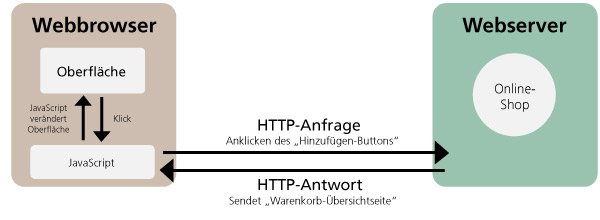
\includegraphics[width=1.0\textwidth]{GrundlagenJavascript.png}
\caption[Grundlagen Javascript]{Funktionsweise von Ajax am Beispiel\protect\footnotemark}
\label{fig:GrundlagendJavascript}
\end{figure}
\footnotetext{Darstellung entnommen von \url{http://www.webmasterpro.de}}